%!TEX root = ../thesis.tex
% ******************************* Thesis Appendix A2 ********************************

\ifpdf
\graphicspath{{chapter-background/Figs/Raster/}{chapter-background/Figs/PDF/}{chapter-background/Figs/}}
\else
\graphicspath{{chapter-background/Figs/Vector/}{chapter-background/Figs/}}
\fi

\section{Background estimation}\label{app:background_estimation}
\begin{figure}[H]
	\centering
	\begin{subfigure}[b]{0.5\linewidth}
		\centering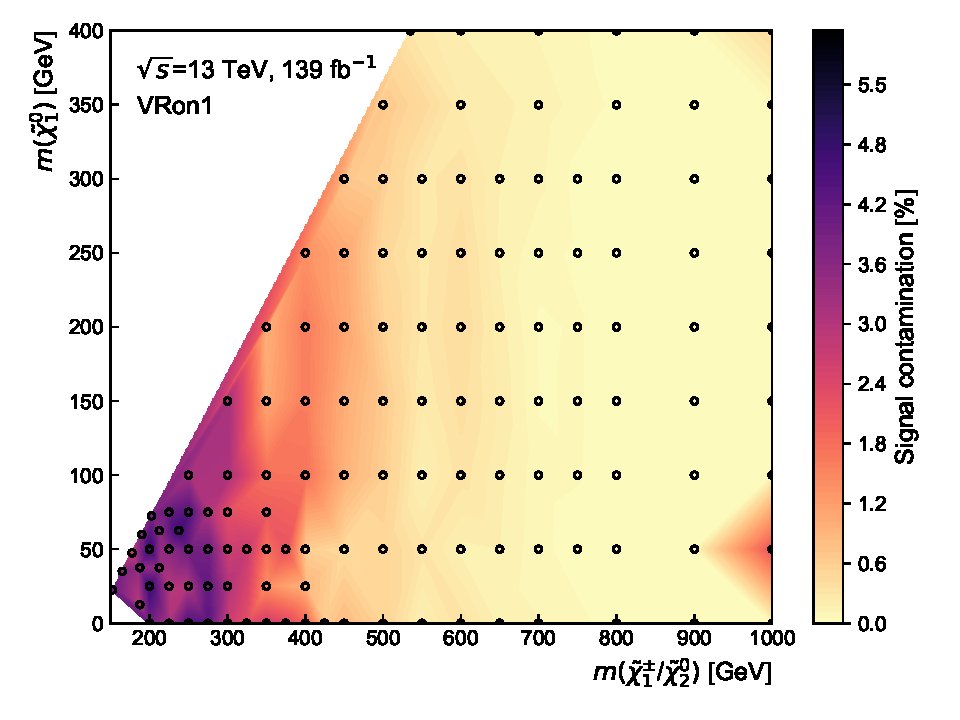
\includegraphics[width=1.0\textwidth]{signal_contamination/plot_VRon1}
		\caption{VR-onLM\label{fig:signal_contamination_VRon1}}
	\end{subfigure}\hfill
	\begin{subfigure}[b]{0.5\linewidth}
		\centering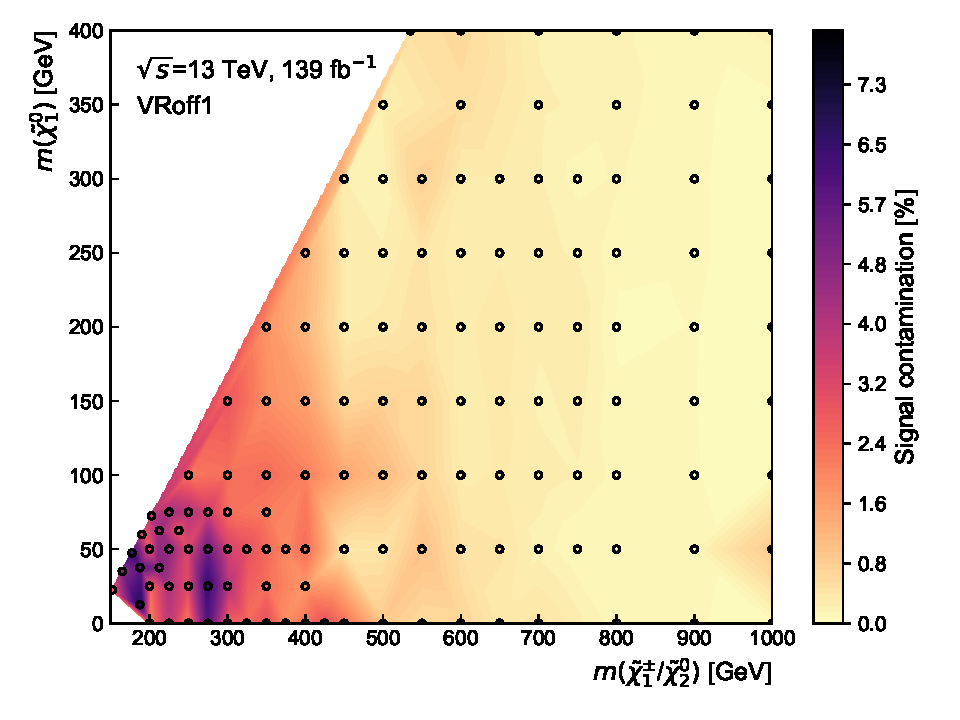
\includegraphics[width=1.0\textwidth]{signal_contamination/plot_VRoff1}
		\caption{VR-offLM\label{fig:signal_contamination_VRoff1}}
	\end{subfigure}\hfill
	\begin{subfigure}[b]{0.5\linewidth}
		\centering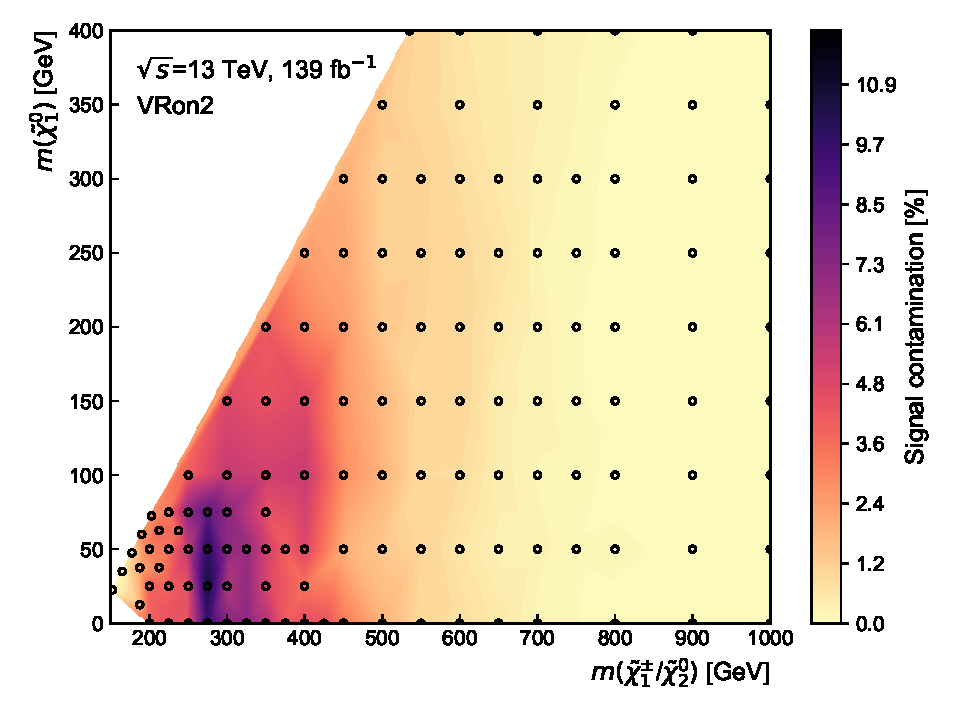
\includegraphics[width=1.0\textwidth]{signal_contamination/plot_VRon2}
		\caption{VR-onMM\label{fig:signal_contamination_VRon2}}
	\end{subfigure}\hfill
	\begin{subfigure}[b]{0.5\linewidth}
		\centering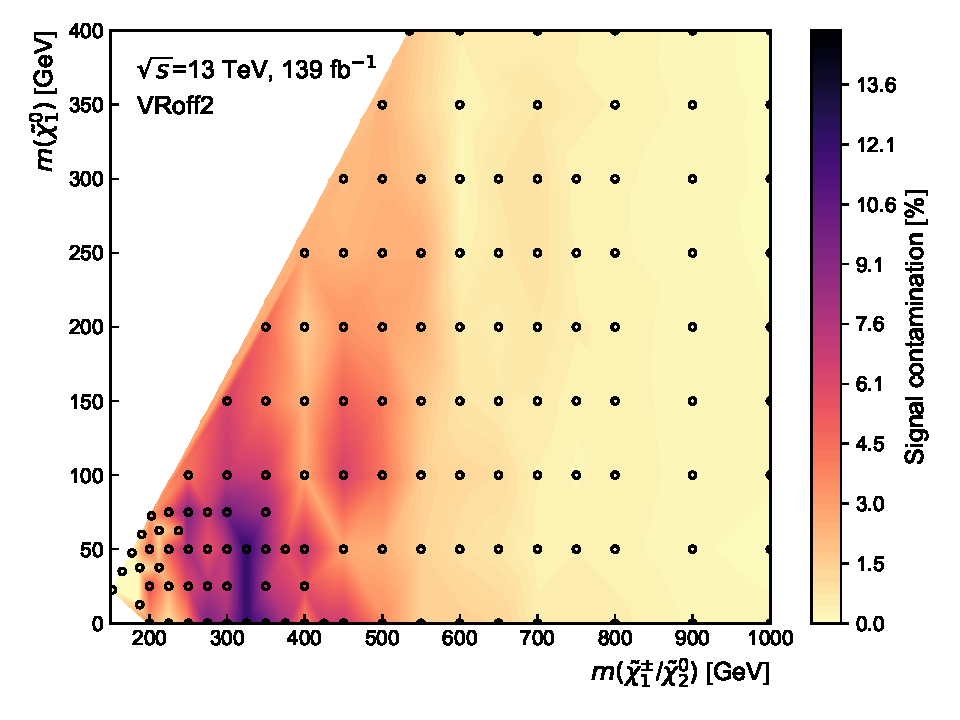
\includegraphics[width=1.0\textwidth]{signal_contamination/plot_VRoff2}
		\caption{VR-offMM\label{fig:signal_contamination_VRoff2}}
	\end{subfigure}\hfill
	\begin{subfigure}[b]{0.5\linewidth}
		\centering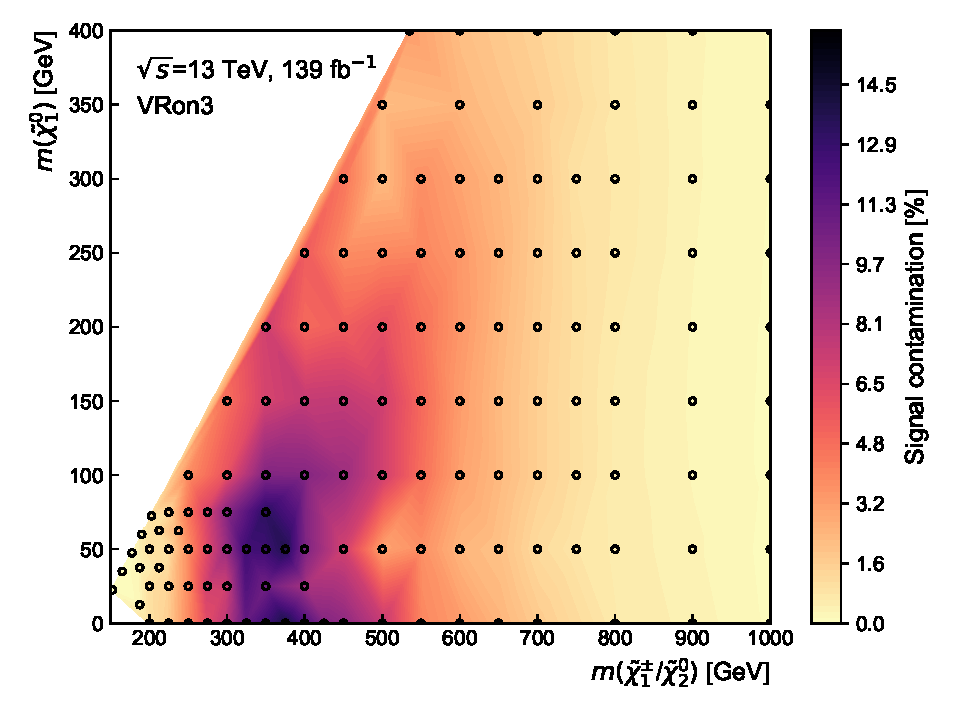
\includegraphics[width=1.0\textwidth]{signal_contamination/plot_VRon3}
		\caption{VR-onHM\label{fig:signal_contaminations_VRon3}}
	\end{subfigure}\hfill
	\begin{subfigure}[b]{0.5\linewidth}
		\centering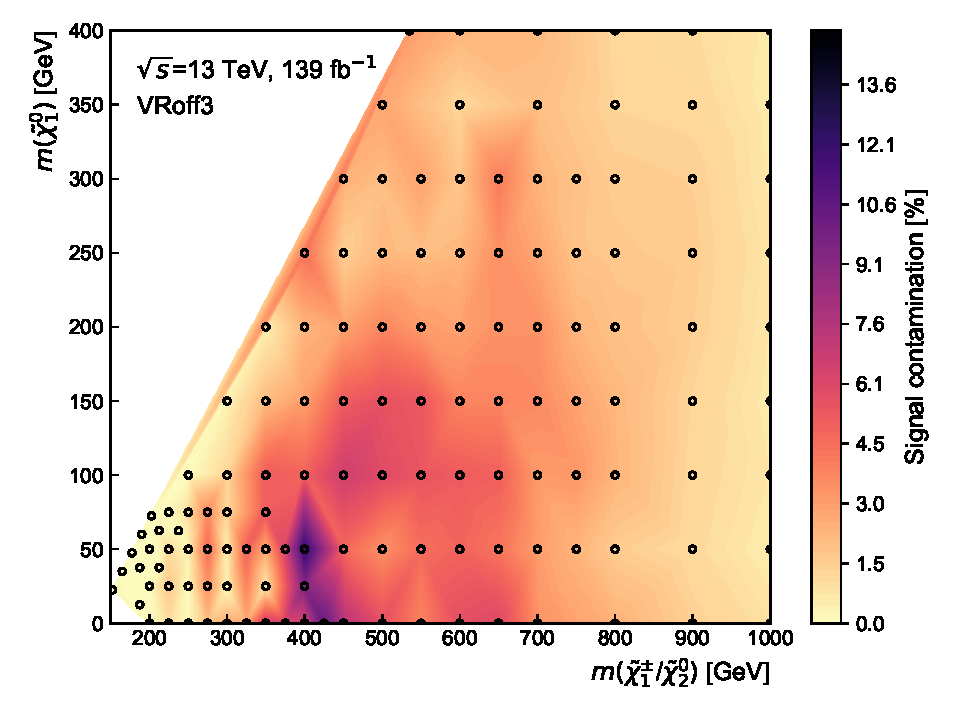
\includegraphics[width=1.0\textwidth]{signal_contamination/plot_VRoff3}
		\caption{VR-offHM\label{fig:signal_contaminations_VRoff3}}
	\end{subfigure}\hfill

	\caption{Signal contamination (shown on the \textit{z-axis}) for all \glspl{vr} throughout the signal grid. The space between the signal points (indicated by the black circles) is interpolated using Delaunay triangles.}
	\label{fig:results_HF_scans}
\end{figure}
